\chapter{Floorplanning Problem}
\label{sec:problem}

In this chapter, the problem is formulated and selected practical applications are introduced.

\section{Problem Formulation}

One of important problems in the branch of industry is the 2D rectangle packing problem, also known as {\em floorplanning} (in the field of digital design). One of possible general assignments is:

\bigskip
\bigskip

{\em Let us have a set of $N$ unoriented rectangles with fixed dimensions. The task is to place all rectangles into the smallest area possible so that they do not overlap. The resulting area is the area of the smallest rectangle that contains all rectangles placed inside.}

\bigskip
\bigskip

This has several practical applications. For example, we can minimise the area of a microchip, thus allowing it running at higher frequency - by placing the most involved (most frequently connected) parts closer to each other, while the electromagnetic characteristics of the circuit may be improved. An automatic instrument that would help with this process by creating at least a good starting point could save a lot of time spent by both expert and beginner digital designers on the design work. 

Another possible application is seen in planning problems, where the rectangle height represents the resource and the width is the time needed. The total cost of the plan is lowest when also the enclosing rectangle is as small as possible. 

Another practical usage (but perhaps not so pleasant) is found in big stores projection. When placing complement goods far from each other, customers spend more money, discovering more tempting goods in the shop.

This kind of problem may be solved by means of evolutionary algorithms - since we can define exact and objective functions for measurement of the solution quality (minimising the connections and the total area). The quality of the placement measured in the proposed algorithm depends on the amount of the {\em unused area} (dead or wasted area), which is simply the total area of the chip without the total area of all modules (in other words, the sum of all areas of the chip which are not covered by any module). However, even more measures are used in literature, for example, the total {\em wire length} or the {\em perimeter} length. Implementation of these measures is easy, and it is not the subject of this work.

The floorplanning problem, as understood in this work, is NP-hard \cite{nphard}, because it is harder than a decision problem {\tt RP(W,H)} (Can the set of modules $M$ be packed on the chip of width $W$ and height $H$?), which was proven in \cite{amir} to be NP-complete.

Every problem assignment consists of a list of modules with fixed integer dimensions (width and height). The modules are not oriented, so they can be rotated freely. Each module has a name which makes identifying of the module in the final result easier. The problem solution provides the exact location of each module and guarantees that no modules overlap. 

\begin{figure}
\centering
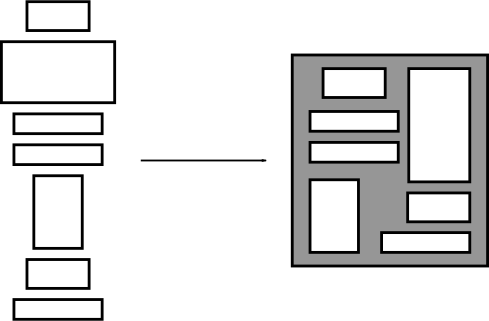
\includegraphics[width=.5\textwidth]{problem}
\caption{An example of the problem and the graphical solution}
\label{fig:problem}
\end{figure}

\begin{figure}
\centering
\subfloat[assignement]{
\begin{minipage}{.45\textwidth}
\centering
module {\tt A} $= 10 \times 20$ \\
module {\tt B} $= 20 \times 50$ \\
module {\tt C} $= 10 \times 50$ \\
module {\tt D} $= 30 \times 20$ \\
\end{minipage}
} \hfill
\subfloat[solution]{
\begin{minipage}{.45\textwidth}
\centering
place module {\tt A} at $(0, 0)$ \\
place module {\tt B} at $(10, 0)$ \\
place module {\tt C} at $(0, 20)$ \\
place module {\tt D} at $(10, 50)$ \\
\end{minipage}
} \\
\caption{Example problem assignment and the solution as the text}
\label{fig:sample}
\end{figure}

\section{Problem Coding}

During the last decade, several different representations were introduced. They differ in the set of floorplans they can encode and in the complexity of the encoding/decoding algorithm. For example, some representations are very compact in size and fast in decoding, but they can represent only a small subset of all possible floorplans.

Usually, we divide floorplans into two categories: The {\em slicing} and {\em non-slicing} floorplans. The slicing floorplans can be represented by a tree, which specifies how the individual modules are put together recursively by binary operations (bottom-up view) or how the final floorplan can be cut down to individual modules (top-down view). The non-slicing floorplans do not have such a property and they are considered as more general and versatile.

The best known slicing floorplan representation is the Polish Expression (PE) \cite{pe} that works with slicing trees. They are very simple to understand and they are convenient, but they may not comprise the optimal solution. Some examples are shown in Fig.~\ref{fig:slicing}. Non-slicing represantitions include a TCG \cite{tcg}, an integrated TCG with a packing sequence (TCG-S) \cite{tcgs}, an O-Tree \cite{otree}, a B*-Tree \cite{btree}, a Corner Block List (CBL) \cite{cbl}, a Sequence Pair (SP) \cite{sp}, and a Bounded Slicing Grid (BSG) \cite{bsg}. Some of the representations listed here are described in more details in the following chapters.

\subsection{Slicing Representation}

\subsubsection{Slicing Tree}

A tree in the area of computer science is a special type of graph used to represent hierarchical structures. Each node in a tree represents an element, and each edge represents the relation `is child of' or `is parent of'. Trees can be also used to represent floorplans that are hierarchical. The best known tree-based representation in floorplanning is probably the {\em slicing tree} written as in {\em postfix expression}.

A slicing tree is a binary tree, where each node has either zero or two descendants (children). Each node represents a certain part of the final floorplan, the so called {\em slice}. Smaller slices can be composed to create bigger slices by using certain binary operations, for example, the {\em vertical join $\oplus$} and the {\em horizontal join $\ominus$}. Each leaf node represents a module to be placed. Each internal node represents a binary operation that puts the slices represented by their children together. And finally, the root of the tree is the biggest slice representing the final floorplan. Some examples are given in Fig.~\ref{fig:slicing}.

The slicing tree is usually encoded as a postfix expression (also known as Polish notation). The postfix expression may be obtained from the slicing tree by its traversion in a post-order (see Fig.~\ref{fig:postorder}). The postfix expression does not need any brackets to retain parenthesis, the associativity is maintained by the positions of the symbols. 

\begin{figure}
\centering
\begin{algorithmic}[1]
  \STATE{traverse left subtree (if any) of current node $ N $ using this function}
  \STATE{traverse right subtree (if any) of current node $ N $ using this function}
  \PRINT{the current node $ N $}
\end{algorithmic}
\caption{The post-order traversion pseudocode}
\label{fig:postorder}
\end{figure}

This representation has many pros and cons. It is very easy to implement because of the recursion contained, the number of the nodes in the tree does not change during the computation, and the search space is small. However, only the slicing floorplans are considered. In case that the optimal floorplan is not slicing, it cannot be found using this representation.

The search space of the slicing tree representation \cite{otree} has the size equal to $O(n!2^{5n-3}/n^{1.5})$. Each floorplan can be encoded using $n(6+\lceil\log n\rceil)$ bits.

However, in the 2001 article by M.~Lai and D.F.~Wong \cite{pe2}, it was proven that by using the slicing tree representation and compaction, all maximally compact placements of modules can be generated. Therefore, under certain conditions, the slicing tree can be considered as a representation for all non-slicing floorplans as well.

\begin{figure}
  \centering
  \subfloat[floorplan 1]{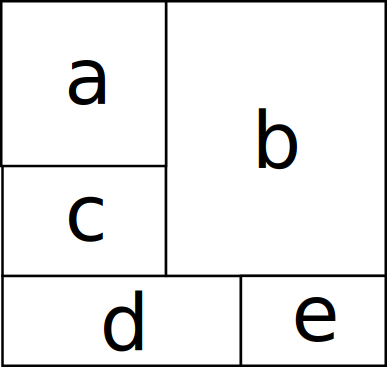
\includegraphics[height=4cm]{slicing1f}} \hspace{1cm}
  \subfloat[slicing tree 1]{\includegraphics[height=4cm]{slicing1t}} \\
  \subfloat[floorplan 2]{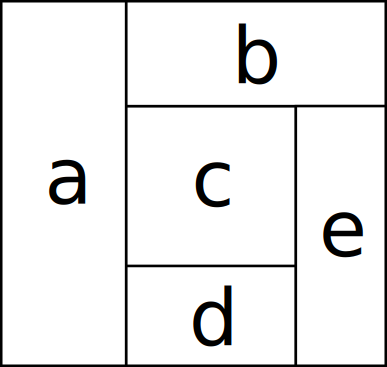
\includegraphics[height=4cm]{slicing2f}} \hspace{1cm}
  \subfloat[slicing tree 2]{\includegraphics[height=4cm]{slicing2t}} \\
  \caption{An example of slicing floorplans and their trees}
  \label{fig:slicing}
\end{figure}

\subsection{Non-Slicing Representations}

\subsubsection{Sequence Pairs}

The sequence pair representation encodes the geometric relations of modules instead of encoding the floorplan structure itself. Let us have a set $M$ of modules. A sequence pair of module set $M$ is a pair of sequences of distinct names of all modules from $M$. For example, for $M = \{a,b,c\}$, the tuple $S = (\mathrm{acb},\mathrm{bac})$ is a valid sequence pair. Each sequence pair specifies the module placement topology by a group of rules, called the {\em horizontal (vertical) constraints}:

$$ S = (\cdots \circ \cdots \bullet \cdots, \cdots \circ \cdots \bullet \cdots) \rightarrow x_\circ + w_\circ \leq x_\bullet $$
$$ S = (\cdots \bullet \cdots \circ \cdots, \cdots \circ \cdots \bullet \cdots) \rightarrow y_\circ + h_\circ \leq y_\bullet $$

A sequence pair is said to be {\em feasible} if there is a feasible packing which satisfies the constraints. Otherwise, it is called {\em infeasible}. It is proven \cite{nphard} that all the sequence pairs for unpositioned modules of fixed size are feasible. An example of a floorplan encoded by the sequence pair is shown in Fig.~\ref{fig:sp}. As we can see from the grid, when the node labels are read left to right, they form the sequence {\tt fcbead}. If they are read top to bottom, they form {\tt ecadfb}.

The search space of the sequence pair representation \cite{otree} has the size equal to $O((n!)^2)$. Each floorplan can be encoded using $2n(\lceil\log n\rceil)$ bits. The solution space always contains the optimal solution, if there is any.

\begin{figure}
\centering
\subfloat[floorplan]{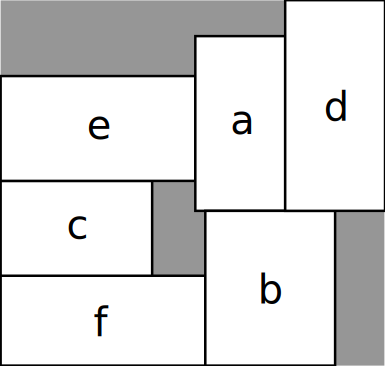
\includegraphics[width=0.45\textwidth]{spf}} \hfill
\subfloat[sequence pair constraints]{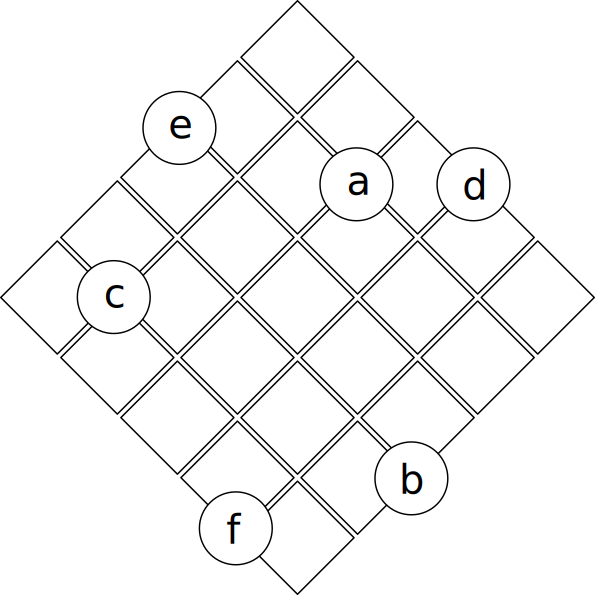
\includegraphics[width=0.45\textwidth]{sp}}
\caption{Example floorplan encoded by a sequence pair $(\mathrm{ecadfb}, \mathrm{fcbead})$}
\label{fig:sp}
\end{figure}

\subsubsection{O-Tree}

The O-Tree representation \cite{otree} can be used in order to represent non-slicing floorplans. The placement can be obtained from an O-Tree in amortized linear time to a number of modules, providing that a special {\em contour} cache structure is used.

An O-Tree is a rooted directed tree in which the order of the subtrees is important. Each O-Tree can be encoded as a tuple $(T, \pi)$, where the $T$ is a bit string of length $2(n-1)$ representing the tree branching structure (0 = step on descending edge, 1 = step on ascending edge) and the $\pi$ is a permutation of modules used for the tree node labeling. The first element in $\pi$ is the tree root. An example of a floorplan encoded by an O-Tree is shown in Fig.~\ref{fig:otree}.

A floorplan is {\em L-compact} if and only if no module can be shifted left without overlapping other modules. A floorplan is {\em B-compact} if and only if no module can be shifted down without overlapping other modules. A floorplan is {\em LB-compact} if and only if it is L-compact and B-compact. A floorplan is {\em admissible} if it is LB-compact. An O-Tree is admissible if the corresponding floorplan is admissible.

Given any placement, there is corresponding LB-compact placement that can be created by a sequence of $x$ direction and $y$ direction compactions. The total area of the resulting LB-compact placement is less or equal to the area of the original placement.  

There is a one to one correspondence between an admissible floorplan and its O-Tree representation.

The search space of an O-Tree representation \cite{otree} has a size of $O(n!2^{2n-2}/n^{1.5})$ (while searching for admissible floorplans only). Each floorplan can be encoded using $n(2+\lceil\log n\rceil)$ bits. The solution space always contains the optimal solution, if any.

\begin{figure}
\centering
\subfloat[floorplan]{\includegraphics[width=0.45\textwidth]{otreef}} \hfill
\subfloat[O-Tree]{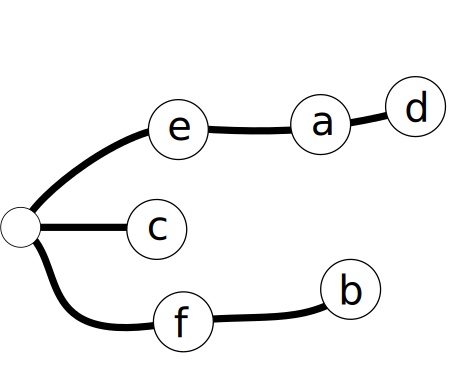
\includegraphics[width=0.45\textwidth]{otree}}
\caption{An example floorplan encoded by an O-Tree $(\mathrm{001101000111}, \mathrm{fbcead})$}
\label{fig:otree}
\end{figure}

\begin{figure}
\centering
\subfloat[whole contour]{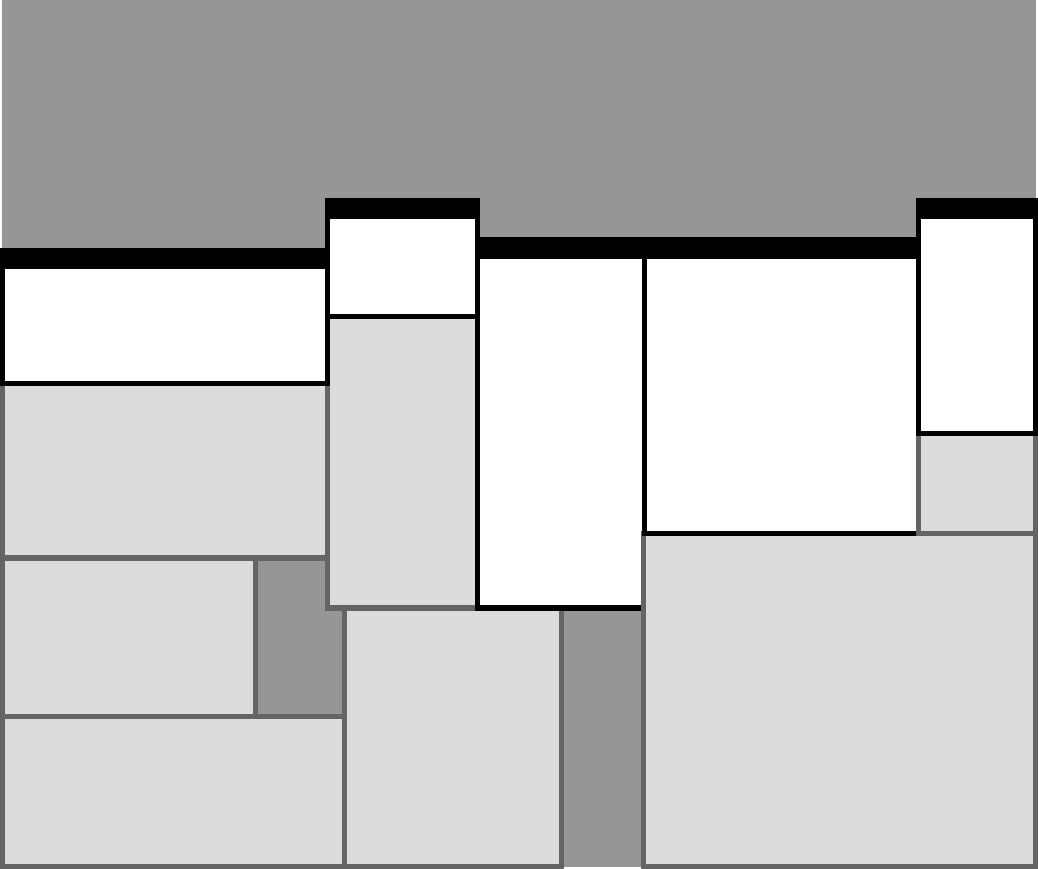
\includegraphics[width=0.45\textwidth]{contour1}} \hfill
\subfloat[contour part evaluated]{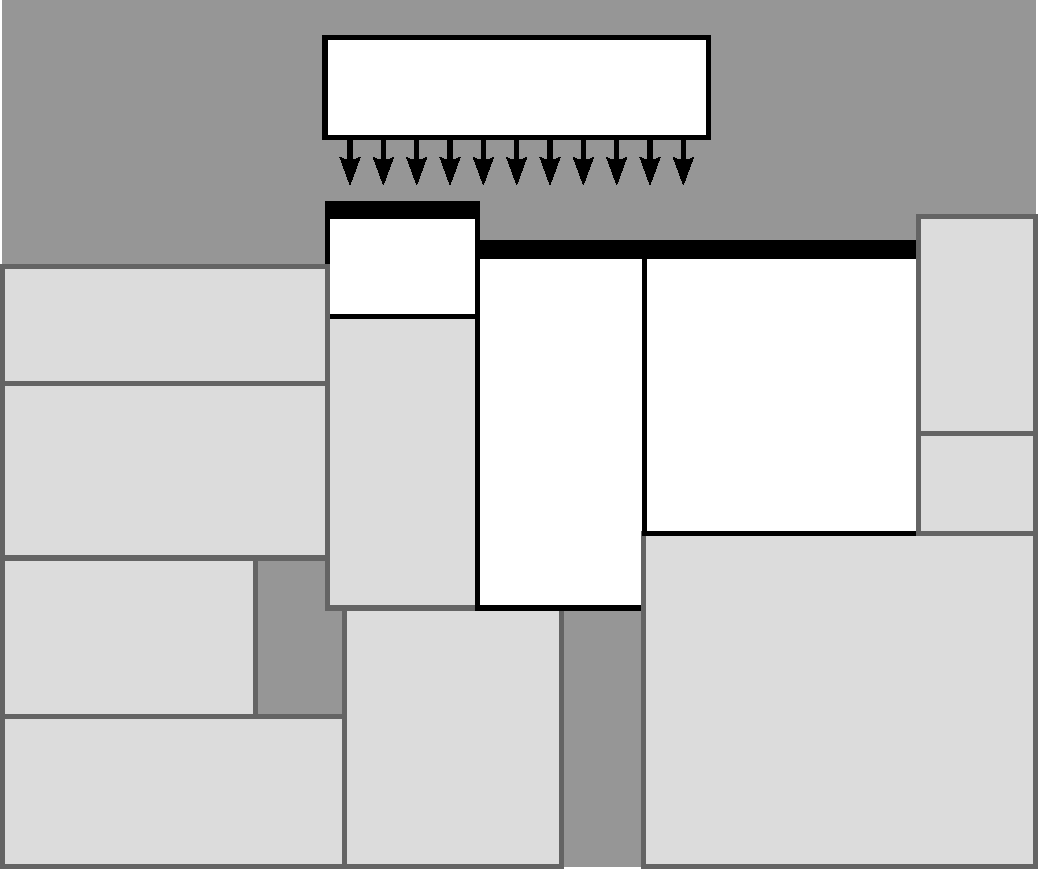
\includegraphics[width=0.45\textwidth]{contour2}}
\caption{The contour structure and its application}
\label{fig:contour}
\end{figure}

\subsubsection{B*-Tree}

The B*-Tree representation \cite{btree} is closely related to the O-Tree representation. It is also based on a tree (binary tree) and uses the similar placement algorithm. In addition, the representation has asymptotically the same number of combinations ($O(n!2^{2n-2}/n^{1.5})$) and uses the same terminology relating the admissible and not admissible floorplans.

The big advantage of the B*-Tree representation is that it is quite simple to add support for general rectilinear modules (encoded as fixed subtrees) or pre-placed modules (nodes in the B*-Tree with position fixed), even soft modules. Furthermore, B*-Tree evaluation can be done incrementally by evaluating the updated subtree only.

The B*-Tree \cite{btree} structure keeps the geometrical relationship between modules as follows. The root is located at $(0, 0)$. If the node $b$ is the left child of the node $a$, the module must be located on the right-hand side and adjacent to the module $a$, that is $x_b = x_a + w_a$. If the node $c$ is the right child of the node $a$, the module must be located above and adjacent to the node $a$, that is $x_c = x_a$. The $y$ coordinate depends on already placed nodes and must be computed as the top-most point of already placed modules that lie under the module newly placed. A special helper contour structure is used in order to speedup this searching.

\begin{figure}
\centering
\subfloat[floorplan]{\includegraphics[width=0.45\textwidth]{btreef}} \hfill
\subfloat[B*-Tree]{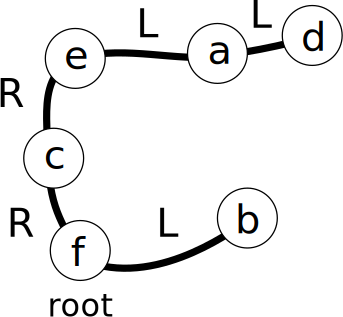
\includegraphics[width=0.45\textwidth]{btree}}
\caption{Example floorplan encoded by a B*-Tree}
\label{fig:btree}
\end{figure}
